\documentclass[border=0pt]{standalone}
\usepackage{times}\usepackage[T1]{fontenc}\usepackage[utf8]{inputenc}\usepackage{amsmath,amssymb,xcolor}
\usepackage{tikz,pgfplots,fontawesome5}
\pgfplotsset{compat=1.18}
\usetikzlibrary{plotmarks,arrows.meta,calc,positioning,shapes.callouts,backgrounds,fit}
\pgfsetplotmarksize{1.7pt}
\tikzset{every picture/.append style={font=\sffamily\scriptsize},
  card/.style={rounded corners=2pt,draw=black!18,fill=black!2,inner sep=3pt,align=left},
  chip/.style={rounded corners=1.5pt,inner sep=1.5pt,font=\sffamily\tiny\bfseries,text=white},
  panel/.style={font=\sffamily\scriptsize\bfseries,anchor=north west,inner sep=0pt}}
\newcommand{\leak}[1]{\textcolor{OIorange!85!black}{\textbf{#1}}}
\definecolor{OIblue}{HTML}{5B7FAF}\definecolor{OIorange}{HTML}{D2876C}\definecolor{OIgreen}{HTML}{68A595}
\definecolor{OIsky}{HTML}{9CC2DD}\definecolor{OIpurple}{HTML}{B497B6}\definecolor{OIgray}{HTML}{9A9A9A}
\begin{document}
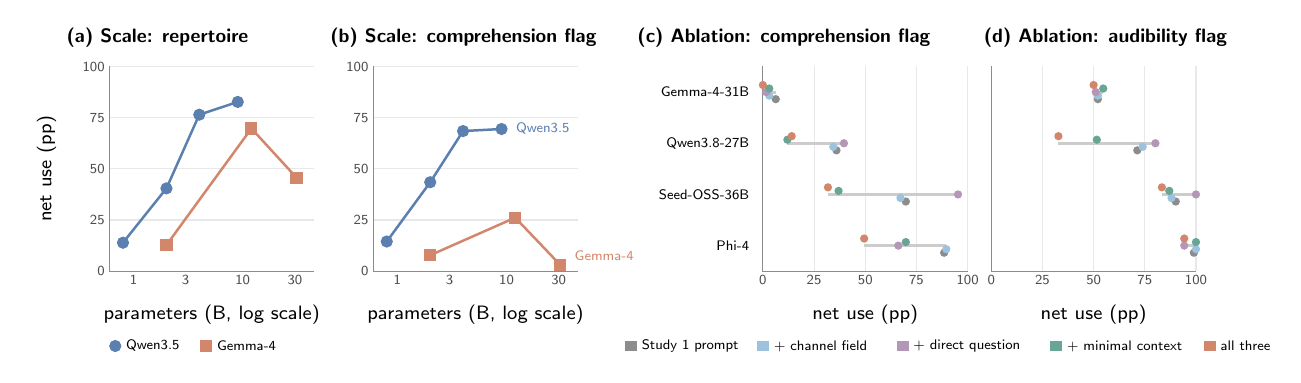
\begin{tikzpicture}[x=1cm,y=1cm]
\begin{scope}[xshift=0.0cm]
\node[panel] at (-0.55,3.10) {(a) Scale: repertoire};
\draw[black!9] (0,0.000)--(2.6,0.000);
\draw[black!9] (0,0.650)--(2.6,0.650);
\draw[black!9] (0,1.300)--(2.6,1.300);
\draw[black!9] (0,1.950)--(2.6,1.950);
\draw[black!9] (0,2.600)--(2.6,2.600);
\draw[black!45,line width=.4pt] (0,2.6)--(0,0)--(2.6,0);
\node[anchor=north,font=\sffamily\tiny,text=black!70,inner sep=1.5pt] at (0.308,0) {1};
\node[anchor=north,font=\sffamily\tiny,text=black!70,inner sep=1.5pt] at (0.969,0) {3};
\node[anchor=north,font=\sffamily\tiny,text=black!70,inner sep=1.5pt] at (1.694,0) {10};
\node[anchor=north,font=\sffamily\tiny,text=black!70,inner sep=1.5pt] at (2.356,0) {30};
\node[anchor=east,font=\sffamily\tiny,text=black!70,inner sep=1.5pt] at (0,0.000) {0};
\node[anchor=east,font=\sffamily\tiny,text=black!70,inner sep=1.5pt] at (0,0.650) {25};
\node[anchor=east,font=\sffamily\tiny,text=black!70,inner sep=1.5pt] at (0,1.300) {50};
\node[anchor=east,font=\sffamily\tiny,text=black!70,inner sep=1.5pt] at (0,1.950) {75};
\node[anchor=east,font=\sffamily\tiny,text=black!70,inner sep=1.5pt] at (0,2.600) {100};
\node[anchor=north,font=\sffamily\scriptsize] at (1.3,-0.3) {parameters (B, log scale)};
\node[anchor=south,rotate=90,font=\sffamily\scriptsize] at (-0.55,1.3) {net use (pp)};
\draw[OIblue,line width=.9pt] (0.173,0.362)--(0.725,1.052)--(1.142,1.988)--(1.631,2.150);
\node[OIblue,inner sep=0pt] at (0.173,0.362) {\pgfuseplotmark{*}};
\node[OIblue,inner sep=0pt] at (0.725,1.052) {\pgfuseplotmark{*}};
\node[OIblue,inner sep=0pt] at (1.142,1.988) {\pgfuseplotmark{*}};
\node[OIblue,inner sep=0pt] at (1.631,2.150) {\pgfuseplotmark{*}};
\draw[OIorange,line width=.9pt] (0.725,0.332)--(1.804,1.813)--(2.376,1.189);
\node[OIorange,inner sep=0pt] at (0.725,0.332) {\pgfuseplotmark{square*}};
\node[OIorange,inner sep=0pt] at (1.804,1.813) {\pgfuseplotmark{square*}};
\node[OIorange,inner sep=0pt] at (2.376,1.189) {\pgfuseplotmark{square*}};
\end{scope}
\begin{scope}[xshift=3.35cm]
\node[panel] at (-0.55,3.10) {(b) Scale: comprehension flag};
\draw[black!9] (0,0.000)--(2.6,0.000);
\draw[black!9] (0,0.650)--(2.6,0.650);
\draw[black!9] (0,1.300)--(2.6,1.300);
\draw[black!9] (0,1.950)--(2.6,1.950);
\draw[black!9] (0,2.600)--(2.6,2.600);
\draw[black!45,line width=.4pt] (0,2.6)--(0,0)--(2.6,0);
\node[anchor=north,font=\sffamily\tiny,text=black!70,inner sep=1.5pt] at (0.308,0) {1};
\node[anchor=north,font=\sffamily\tiny,text=black!70,inner sep=1.5pt] at (0.969,0) {3};
\node[anchor=north,font=\sffamily\tiny,text=black!70,inner sep=1.5pt] at (1.694,0) {10};
\node[anchor=north,font=\sffamily\tiny,text=black!70,inner sep=1.5pt] at (2.356,0) {30};
\node[anchor=east,font=\sffamily\tiny,text=black!70,inner sep=1.5pt] at (0,0.000) {0};
\node[anchor=east,font=\sffamily\tiny,text=black!70,inner sep=1.5pt] at (0,0.650) {25};
\node[anchor=east,font=\sffamily\tiny,text=black!70,inner sep=1.5pt] at (0,1.300) {50};
\node[anchor=east,font=\sffamily\tiny,text=black!70,inner sep=1.5pt] at (0,1.950) {75};
\node[anchor=east,font=\sffamily\tiny,text=black!70,inner sep=1.5pt] at (0,2.600) {100};
\node[anchor=north,font=\sffamily\scriptsize] at (1.3,-0.3) {parameters (B, log scale)};
\draw[OIblue,line width=.9pt] (0.173,0.377)--(0.725,1.130)--(1.142,1.780)--(1.631,1.806);
\node[OIblue,inner sep=0pt] at (0.173,0.377) {\pgfuseplotmark{*}};
\node[OIblue,inner sep=0pt] at (0.725,1.130) {\pgfuseplotmark{*}};
\node[OIblue,inner sep=0pt] at (1.142,1.780) {\pgfuseplotmark{*}};
\node[OIblue,inner sep=0pt] at (1.631,1.806) {\pgfuseplotmark{*}};
\node[anchor=west,font=\sffamily\tiny,text=OIblue] at (1.691,1.806) {Qwen3.5};
\draw[OIorange,line width=.9pt] (0.725,0.203)--(1.804,0.680)--(2.376,0.081);
\node[OIorange,inner sep=0pt] at (0.725,0.203) {\pgfuseplotmark{square*}};
\node[OIorange,inner sep=0pt] at (1.804,0.680) {\pgfuseplotmark{square*}};
\node[OIorange,inner sep=0pt] at (2.376,0.081) {\pgfuseplotmark{square*}};
\node[anchor=west,font=\sffamily\tiny,text=OIorange] at (2.436,0.201) {Gemma-4};
\end{scope}
\begin{scope}[xshift=8.3cm]
\node[panel] at (-1.6,3.10) {(c) Ablation: comprehension flag};
\draw[black!9] (0.000,0)--(0.000,2.6);
\draw[black!9] (0.650,0)--(0.650,2.6);
\draw[black!9] (1.300,0)--(1.300,2.6);
\draw[black!9] (1.950,0)--(1.950,2.6);
\draw[black!9] (2.600,0)--(2.600,2.6);
\draw[black!45,line width=.4pt] (0,2.6)--(0,0)--(2.6,0);
\node[anchor=north,font=\sffamily\tiny,text=black!70,inner sep=1.5pt] at (0.000,0) {0};
\node[anchor=north,font=\sffamily\tiny,text=black!70,inner sep=1.5pt] at (0.650,0) {25};
\node[anchor=north,font=\sffamily\tiny,text=black!70,inner sep=1.5pt] at (1.300,0) {50};
\node[anchor=north,font=\sffamily\tiny,text=black!70,inner sep=1.5pt] at (1.950,0) {75};
\node[anchor=north,font=\sffamily\tiny,text=black!70,inner sep=1.5pt] at (2.600,0) {100};
\node[anchor=north,font=\sffamily\scriptsize] at (1.3,-0.3) {net use (pp)};
\node[anchor=east,font=\sffamily\tiny] at (-0.05,2.275) {Gemma-4-31B};
\draw[black!20,line width=1.1pt] (0.000,2.275)--(0.163,2.275);
\fill[black!45] (0.163,2.185) circle (1.5pt);
\fill[OIsky] (0.081,2.230) circle (1.5pt);
\fill[OIpurple] (0.041,2.275) circle (1.5pt);
\fill[OIgreen] (0.081,2.320) circle (1.5pt);
\fill[OIorange] (0.000,2.365) circle (1.5pt);
\node[anchor=east,font=\sffamily\tiny] at (-0.05,1.625) {Qwen3.8-27B};
\draw[black!20,line width=1.1pt] (0.311,1.625)--(1.029,1.625);
\fill[black!45] (0.934,1.535) circle (1.5pt);
\fill[OIsky] (0.894,1.580) circle (1.5pt);
\fill[OIpurple] (1.029,1.625) circle (1.5pt);
\fill[OIgreen] (0.311,1.670) circle (1.5pt);
\fill[OIorange] (0.366,1.715) circle (1.5pt);
\node[anchor=east,font=\sffamily\tiny] at (-0.05,0.975) {Seed-OSS-36B};
\draw[black!20,line width=1.1pt] (0.826,0.975)--(2.478,0.975);
\fill[black!45] (1.815,0.885) circle (1.5pt);
\fill[OIsky] (1.747,0.930) circle (1.5pt);
\fill[OIpurple] (2.478,0.975) circle (1.5pt);
\fill[OIgreen] (0.961,1.020) circle (1.5pt);
\fill[OIorange] (0.826,1.065) circle (1.5pt);
\node[anchor=east,font=\sffamily\tiny] at (-0.05,0.325) {Phi-4};
\draw[black!20,line width=1.1pt] (1.286,0.325)--(2.329,0.325);
\fill[black!45] (2.302,0.235) circle (1.5pt);
\fill[OIsky] (2.329,0.280) circle (1.5pt);
\fill[OIpurple] (1.720,0.325) circle (1.5pt);
\fill[OIgreen] (1.815,0.370) circle (1.5pt);
\fill[OIorange] (1.286,0.415) circle (1.5pt);
\end{scope}
\begin{scope}[xshift=11.2cm]
\node[panel] at (-0.1,3.10) {(d) Ablation: audibility flag};
\draw[black!9] (0.000,0)--(0.000,2.6);
\draw[black!9] (0.650,0)--(0.650,2.6);
\draw[black!9] (1.300,0)--(1.300,2.6);
\draw[black!9] (1.950,0)--(1.950,2.6);
\draw[black!9] (2.600,0)--(2.600,2.6);
\draw[black!45,line width=.4pt] (0,2.6)--(0,0)--(2.6,0);
\node[anchor=north,font=\sffamily\tiny,text=black!70,inner sep=1.5pt] at (0.000,0) {0};
\node[anchor=north,font=\sffamily\tiny,text=black!70,inner sep=1.5pt] at (0.650,0) {25};
\node[anchor=north,font=\sffamily\tiny,text=black!70,inner sep=1.5pt] at (1.300,0) {50};
\node[anchor=north,font=\sffamily\tiny,text=black!70,inner sep=1.5pt] at (1.950,0) {75};
\node[anchor=north,font=\sffamily\tiny,text=black!70,inner sep=1.5pt] at (2.600,0) {100};
\node[anchor=north,font=\sffamily\scriptsize] at (1.3,-0.3) {net use (pp)};
\draw[black!20,line width=1.1pt] (1.300,2.275)--(1.422,2.275);
\fill[black!45] (1.354,2.185) circle (1.5pt);
\fill[OIsky] (1.354,2.230) circle (1.5pt);
\fill[OIpurple] (1.327,2.275) circle (1.5pt);
\fill[OIgreen] (1.422,2.320) circle (1.5pt);
\fill[OIorange] (1.300,2.365) circle (1.5pt);
\draw[black!20,line width=1.1pt] (0.853,1.625)--(2.085,1.625);
\fill[black!45] (1.855,1.535) circle (1.5pt);
\fill[OIsky] (1.923,1.580) circle (1.5pt);
\fill[OIpurple] (2.085,1.625) circle (1.5pt);
\fill[OIgreen] (1.341,1.670) circle (1.5pt);
\fill[OIorange] (0.853,1.715) circle (1.5pt);
\draw[black!20,line width=1.1pt] (2.167,0.975)--(2.600,0.975);
\fill[black!45] (2.343,0.885) circle (1.5pt);
\fill[OIsky] (2.289,0.930) circle (1.5pt);
\fill[OIpurple] (2.600,0.975) circle (1.5pt);
\fill[OIgreen] (2.261,1.020) circle (1.5pt);
\fill[OIorange] (2.167,1.065) circle (1.5pt);
\draw[black!20,line width=1.1pt] (2.451,0.325)--(2.600,0.325);
\fill[black!45] (2.573,0.235) circle (1.5pt);
\fill[OIsky] (2.600,0.280) circle (1.5pt);
\fill[OIpurple] (2.451,0.325) circle (1.5pt);
\fill[OIgreen] (2.600,0.370) circle (1.5pt);
\fill[OIorange] (2.451,0.415) circle (1.5pt);
\end{scope}
\node[OIblue,inner sep=0pt] at (0.075,-0.950) {\pgfuseplotmark{*}};
\node[anchor=west,font=\sffamily\tiny,inner sep=1pt] at (0.170,-0.950) {Qwen3.5};
\node[OIorange,inner sep=0pt] at (1.230,-0.950) {\pgfuseplotmark{square*}};
\node[anchor=west,font=\sffamily\tiny,inner sep=1pt] at (1.325,-0.950) {Gemma-4};
\fill[black!45] (6.550,-1.010) rectangle (6.700,-0.890);
\node[anchor=west,font=\sffamily\tiny,inner sep=1pt] at (6.720,-0.950) {Study 1 prompt};
\fill[OIsky] (8.230,-1.010) rectangle (8.380,-0.890);
\node[anchor=west,font=\sffamily\tiny,inner sep=1pt] at (8.400,-0.950) {+ channel field};
\fill[OIpurple] (10.000,-1.010) rectangle (10.150,-0.890);
\node[anchor=west,font=\sffamily\tiny,inner sep=1pt] at (10.170,-0.950) {+ direct question};
\fill[OIgreen] (11.950,-1.010) rectangle (12.100,-0.890);
\node[anchor=west,font=\sffamily\tiny,inner sep=1pt] at (12.120,-0.950) {+ minimal context};
\fill[OIorange] (13.900,-1.010) rectangle (14.050,-0.890);
\node[anchor=west,font=\sffamily\tiny,inner sep=1pt] at (14.070,-0.950) {all three};
\end{tikzpicture}
\end{document}
